
%% modelo.tex
%% V1.0
%% 03/05/2009
%% Hugo Vieira Neto
%%
%% Modelo de artigo de conferência IEEE para LaTeX
%% Requer os arquivos IEEEtran.cls, IEEEtran.bst e IEEEabrv.bib

% *** PREÂMBULO ***
\documentclass[conference,peerreview]{IEEEtran}
% Na versão final do artigo, a opção peerreview deve ser removida para
% que as informações sobre os autores fiquem aparentes após o título.

% Pacotes para a utilização da língua portuguesa.
\usepackage[brazil]{babel}
\usepackage[utf8]{inputenc}
% As linhas acima devem ser comentadas se o artigo for escrito em inglês.

% Pacotes para o uso de equações e símbolos matemáticos.
\usepackage[cmex10]{amsmath}
\usepackage{amsfonts,amssymb}

% Pacotes para o uso de tabelas, gráficos e subfiguras.
\usepackage{array}
\usepackage{graphicx}
\usepackage[caption=false,font=footnotesize]{subfig}

% Pacote para a formatação ordenada automática de múltiplas citações.
\usepackage{cite}

% Pacote para a formatação adequada de URL.
\usepackage{url}

% Falhas de separação em sílabas devem ser listadas aqui
\hyphenation{}


% *** CORPO DO TEXTO ***
\begin{document}

% Título do artigo
\title{Aprendizado de máquinas e Espectroscopia Raman para identificação de fungos}
% Quebras de linha \\ podem ser inseridas para melhor formatação de títulos
% longos.


% Nome e afiliação do autor
\author{
	\IEEEauthorblockN{Daniel Silva Costa}
	\IEEEauthorblockA{
		CPGEI / UTFPR\\
		Avenida Sete de Setembro, 3165\\
		Curitiba-PR - CEP 80.230-910\\
		E-mail: eng.daniels.costa@gmail.com\\
		\url{https://github.com/danielscosta}
	} % \IEEEauthorblockA
} % \author
% Para múltiplos autores e afiliações, consultar exemplos no arquivo
% bare_conf.tex


% Formatação do título e autoria do artigo. Em artigos com a opção peerreview,
% a autoria é ocultada e as páginas são numeradas.
\ifCLASSOPTIONpeerreview
	\setcounter{page}{1}
	\IEEEpeerreviewmaketitle
\else
	\maketitle
\fi


% Resumo do artigo
\begin{abstract}
A identificação da espécie de um fungo causador de doenças é determinante na escolha do tratamento mais adequado. Contudo tal tarefa pode ser desafiadora dada as semelhanças entre as espécies. Para tanto, pode ser utilizado o sequenciamento genético, entretanto, é uma técnica de elevado custo e requer equipamentos que não estão facilmente disponíveis.
Este trabalho apresenta uma proposta de projeto para analisar dados do espectro Raman de algumas espécies de fungos através de técnicas de aprendizado de máquinas, de forma que, consiga-se identificar quais dados são relevantes para diferenciação e identificação de uma espécie específica dentre as analisadas. 
\end{abstract}

\section{Introdução}
O Reino Fungi é composto pelas mais variadas formas de seres, desde micro-organismos até cogumelos. Contudo, quando deseja-se diferenciar espécies de mesmo gênero (táxon da classificação biológica) isto torna-se uma tarefa árdua, pois tais diferenças só são perceptíveis nas estruturas celulares destes seres, como pode ser verificado na figura \ref{fg_exemp1}.

\begin{figure}[ht]
\centering
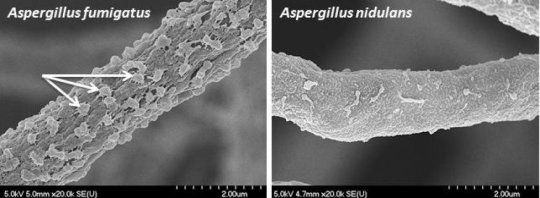
\includegraphics[width=7.5cm]{fungus_dif}
\caption{Diferença nas estruturas celulares das espécies fungos fumigatus e nidulans ambos do gênero Aspergillus. Crédito: Lee et al. The Fungal Exopolysaccharide Galactosaminogalactan Mediates Virulence by Enhancing Resistance to Neutrophil Extracellular Traps. PLOS Pathogens, 2015; 11 (10): e1005187}
\label{fg_exemp1}
\end{figure}

Realizar o sequênciamento genético de uma amostra de células de um fungu é a forma mais assertiva de determinar a qual espécie o mesmo pertence. Mas, é um método com alto custo e requer um sequenciador genético a disposição. Por isto este trabalho propoe utilizar-se de dados de Espectroscopia Raman das células dos fungos para criar uma modelo de aprendizagem de máquina capaz de identificar a espécie de um fungo.

Nas próximas sessões deste trabalho serão detalhadas a significância do sinal da Espectroscopia Raman para o caso de estudo, técnicas de aprendizado de Máquina como PCA(Principal Component Analysis) e Feature Selection e será proposta uma discussão do porquê estas técnicas podem trazer um valor significante a materia de estudo, além de apresentar os resultados esperados ao fim desta pesquisa.

\section{Revisão da literatura}

\section{Materiais e métodos}

\section{Discussão e resultados esperados}
\section{Conclusão}


\section*{Reconhecimento}

\bibliographystyle{IEEEtran}
\bibliography{IEEEabrv,modref}

\end{document}